% Generated by build_candidate_figures.py; review-only figure options.
\clearpage
\section*{Additional figure candidates for review}
These optional figures expand the analyses discussed in the HTML report using corrected archived data. They are included for figure selection, not as a proposed final figure count. The four main figures remain unchanged. Core analyses retain the single 0.75~\AA{} recovery cutoff; drug analyses remain exploratory. Historical energy and random-subsampling analyses are excluded.
\begingroup
\renewcommand{\thefigure}{C\ifnum\value{figure}<10 0\fi\arabic{figure}}
\setcounter{figure}{0}
\clearpage
\begin{figure}[p]
\centering
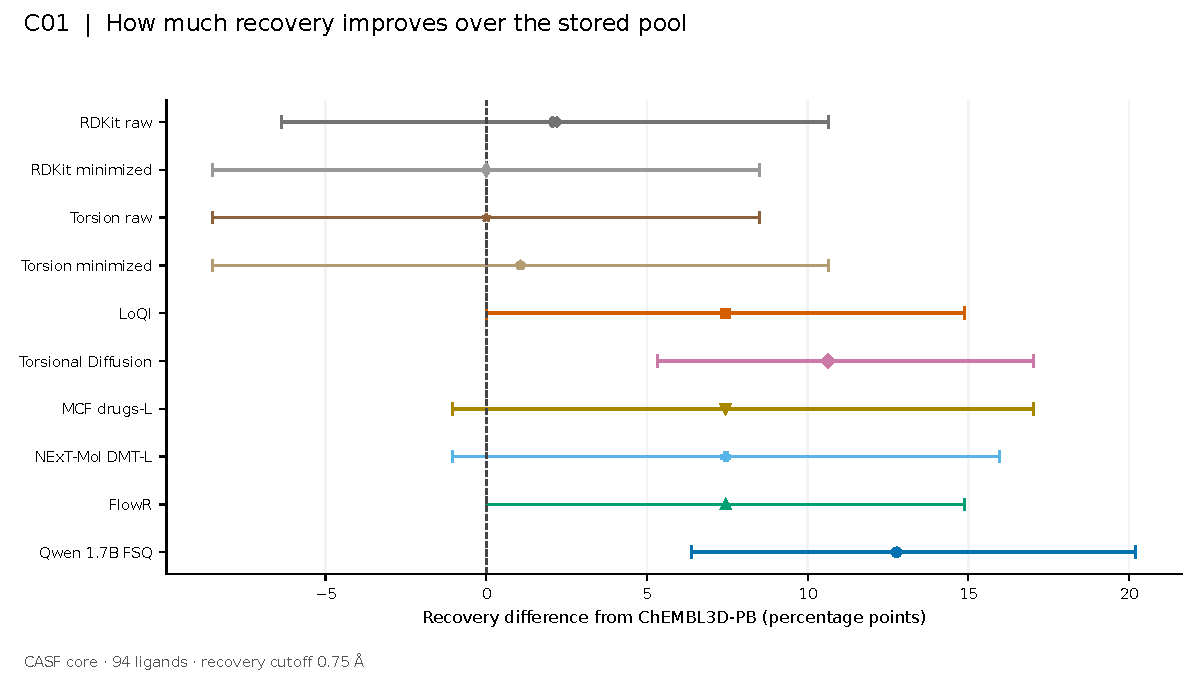
\includegraphics[width=\linewidth,height=0.72\textheight,keepaspectratio]{figures/candidates/c01-paired-recovery.pdf}
\caption{\textbf{How much recovery improves over the stored pool.} Paired differences in core recovery between each 1,000-candidate pipeline and the finite stored ChEMBL3D-PB pool. Error bars are exploratory 95\% percentile intervals from 10,000 paired bootstrap resamples of the 94 core entries (94 distinct parent compounds; seed 20260928). Missing outputs are misses. The comparison does not match retained count or computing cost, and intervals are not adjusted for multiple comparisons or checkpoint selection.}
\label{fig:candidate-c01-paired-recovery}
\end{figure}
\clearpage
\begin{figure}[p]
\centering
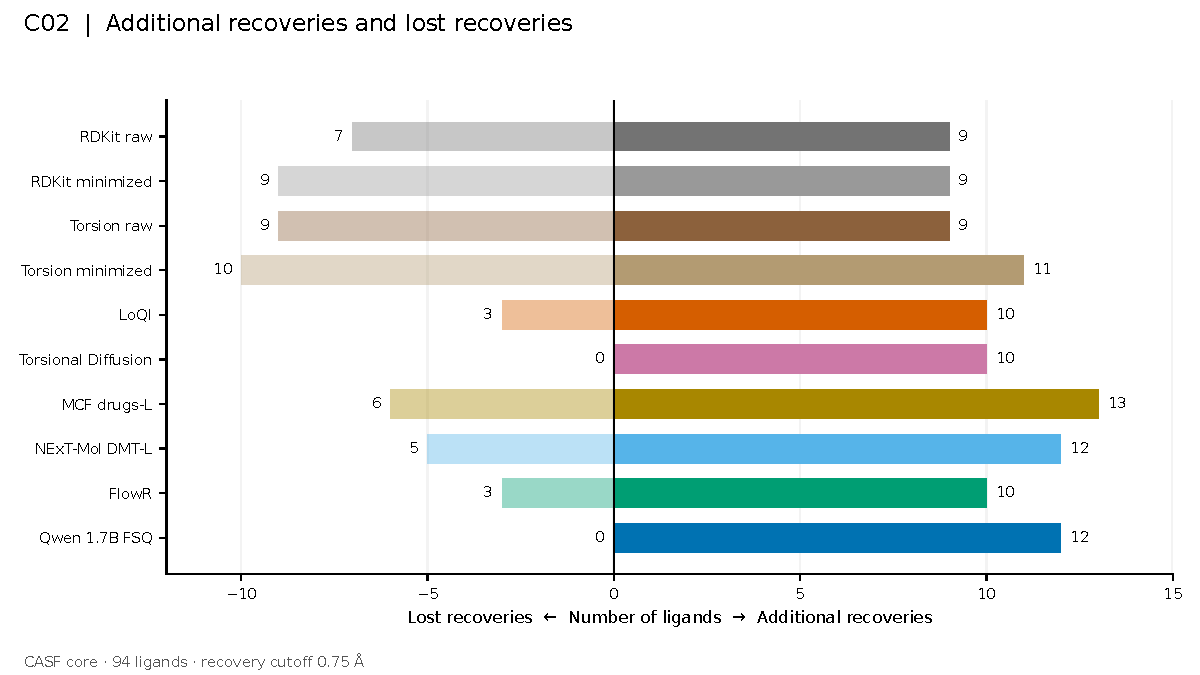
\includegraphics[width=\linewidth,height=0.72\textheight,keepaspectratio]{figures/candidates/c02-gained-lost.pdf}
\caption{\textbf{Additional recoveries and lost recoveries.} Numbers of core ligands recovered only by a generated pool (right) or only by ChEMBL3D-PB (left). Shared hits and shared misses are omitted. Generated pools use the 1,000-candidate target and PoseBusters filtering; the reference is the finite stored pool. A positive net difference need not imply improvement on every ligand.}
\label{fig:candidate-c02-gained-lost}
\end{figure}
\clearpage
\begin{figure}[p]
\centering
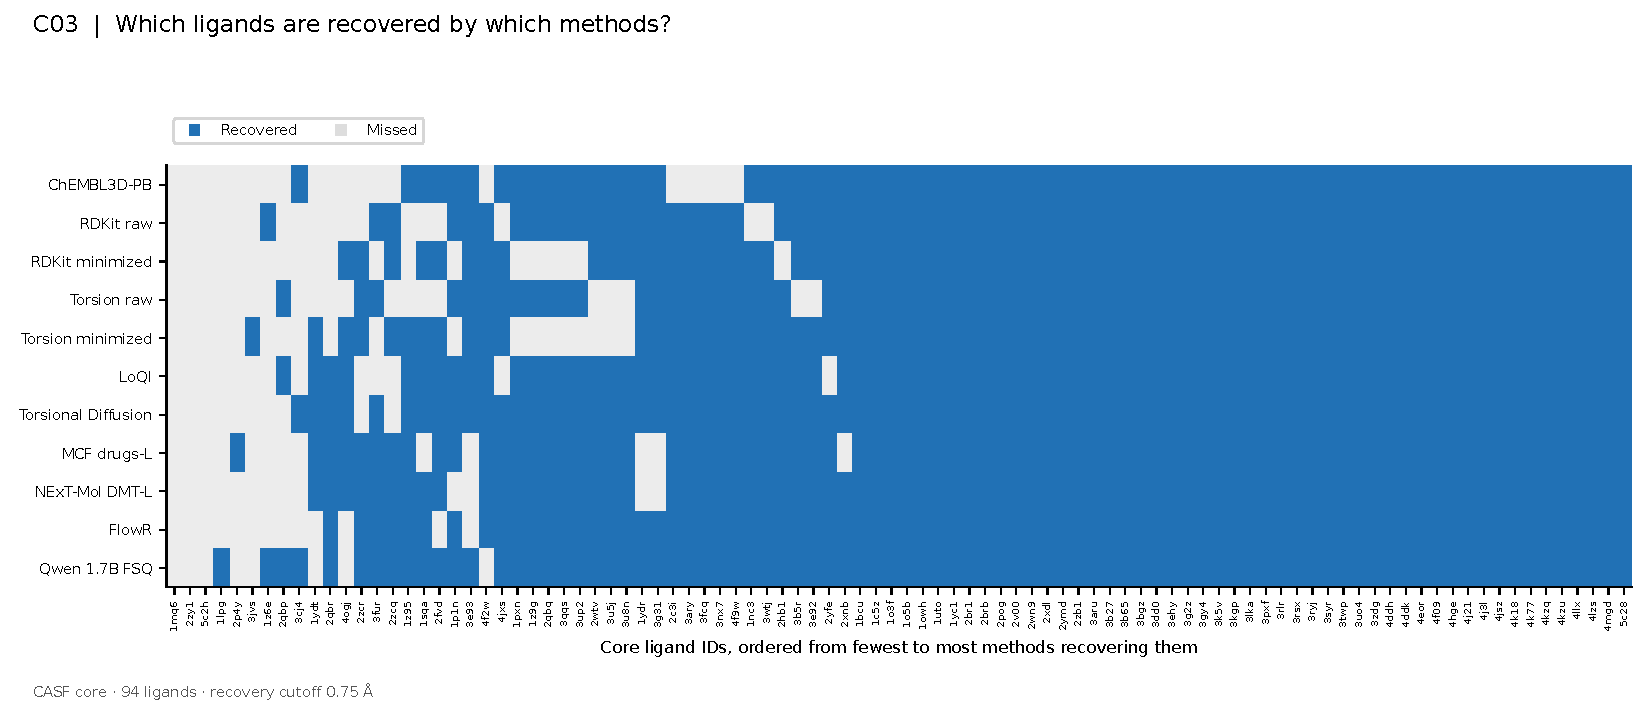
\includegraphics[width=\linewidth,height=0.72\textheight,keepaspectratio]{figures/candidates/c03-ligand-recovery.pdf}
\caption{\textbf{Which ligands are recovered by which methods?.} Binary recovery for every core ligand and each of the ten generation pipelines plus ChEMBL3D-PB. Blue cells indicate a PoseBusters-passing conformer within 0.75~\AA{}; gray cells indicate a miss, including missing output. Columns are sorted by the number of methods recovering each ligand. Generated pools use the 1,000-candidate target. This is a descriptive map of correlated outcomes, not an independent set of method trials.}
\label{fig:candidate-c03-ligand-recovery}
\end{figure}
\clearpage
\begin{figure}[p]
\centering
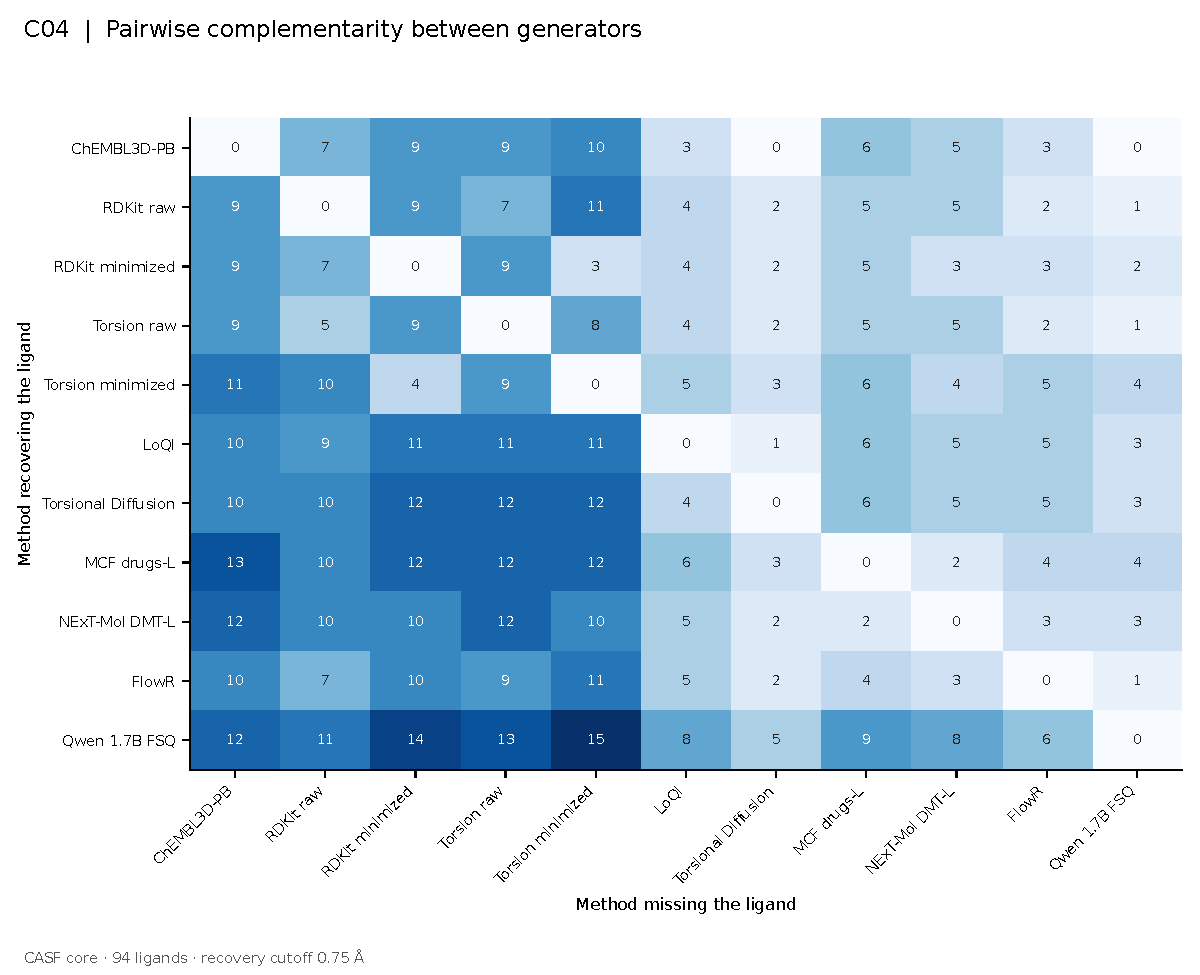
\includegraphics[width=\linewidth,height=0.72\textheight,keepaspectratio]{figures/candidates/c04-complementarity.pdf}
\caption{\textbf{Pairwise complementarity between generators.} Each cell counts ligands recovered by the row method and missed by the column method. The matrix is directional; its diagonal is zero. Generated pools use 1,000 candidates before filtering, while ChEMBL3D-PB uses its stored pool. Counts identify complementary recovery patterns; they do not measure the performance or cost of a newly generated mixed ensemble.}
\label{fig:candidate-c04-complementarity}
\end{figure}
\clearpage
\begin{figure}[p]
\centering
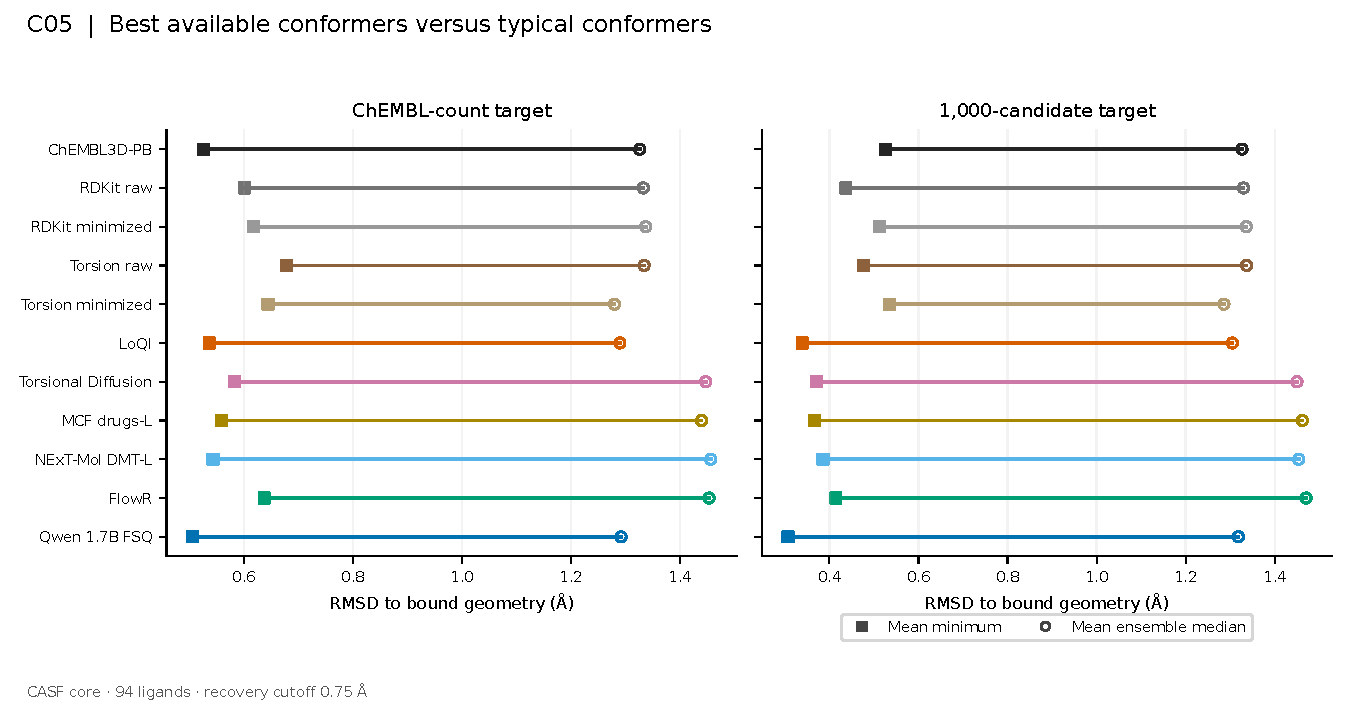
\includegraphics[width=\linewidth,height=0.72\textheight,keepaspectratio]{figures/candidates/c05-best-typical.pdf}
\caption{\textbf{Best available conformers versus typical conformers.} Mean per-ligand minimum RMSD (filled squares) and mean per-ligand ensemble-median RMSD (open circles), at both candidate targets. These continuous distances are conditional on measurable ensembles, unlike recovery fractions, whose denominator includes all 94 core entries. ChEMBL3D-PB is the same stored pool in both panels. Connecting segments indicate the difference between two summaries, not confidence intervals or paired transformations.}
\label{fig:candidate-c05-best-typical}
\end{figure}
\clearpage
\begin{figure}[p]
\centering
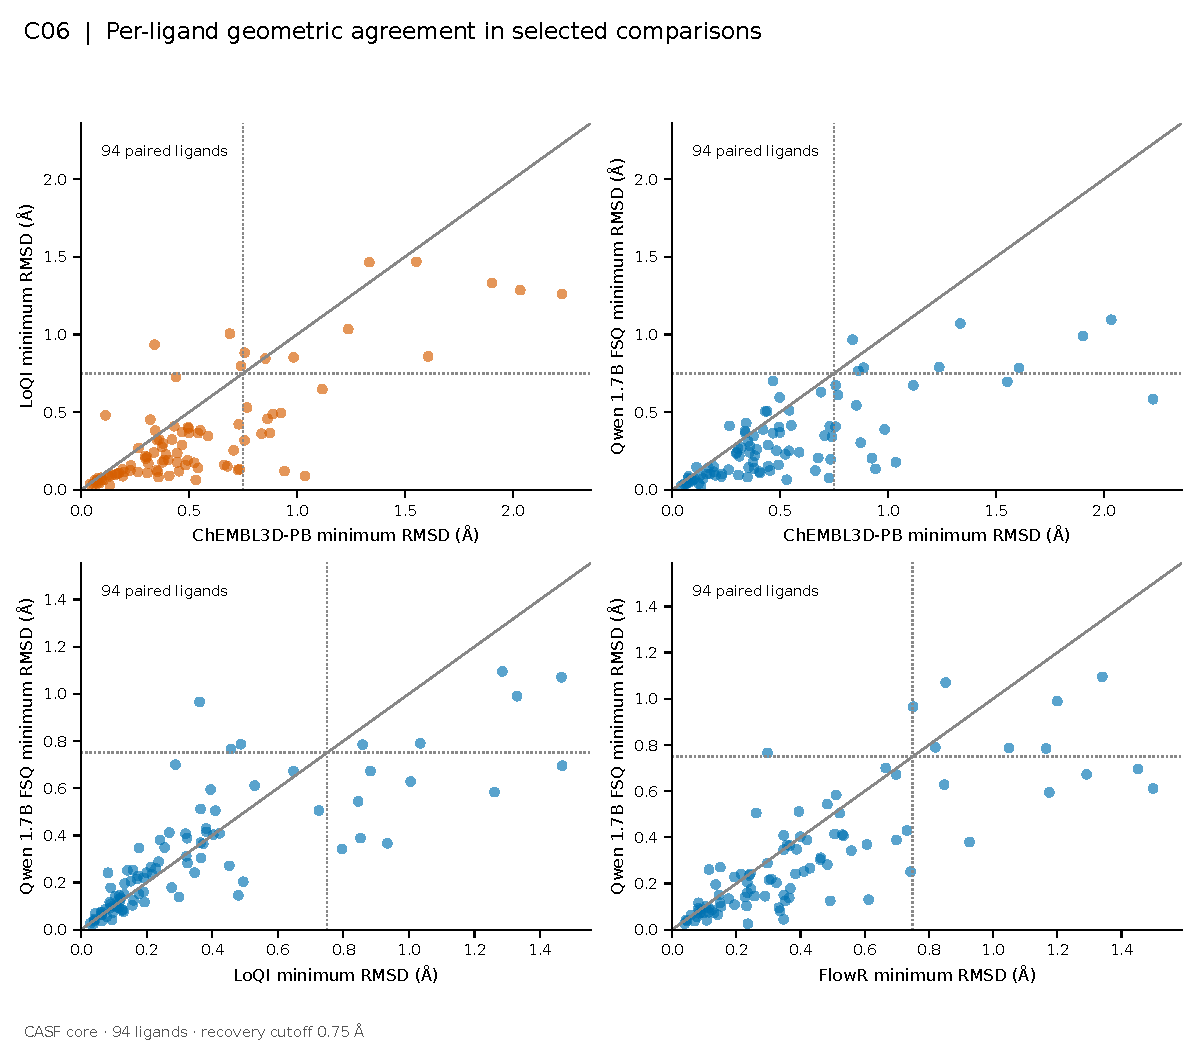
\includegraphics[width=\linewidth,height=0.72\textheight,keepaspectratio]{figures/candidates/c06-paired-rmsd.pdf}
\caption{\textbf{Per-ligand geometric agreement in selected comparisons.} Minimum RMSD for paired measurable core ensembles in four selected comparisons. Each point is one ligand; the diagonal indicates equal distance and dotted lines mark the sole recovery cutoff, 0.75~\AA{}. Lower values are better. Points below the diagonal favor the vertical-axis method. Generated pools use 1,000 candidates before filtering. Panel-specific sample counts exclude unmeasurable pairs; they are not the recovery denominator.}
\label{fig:candidate-c06-paired-rmsd}
\end{figure}
\clearpage
\begin{figure}[p]
\centering
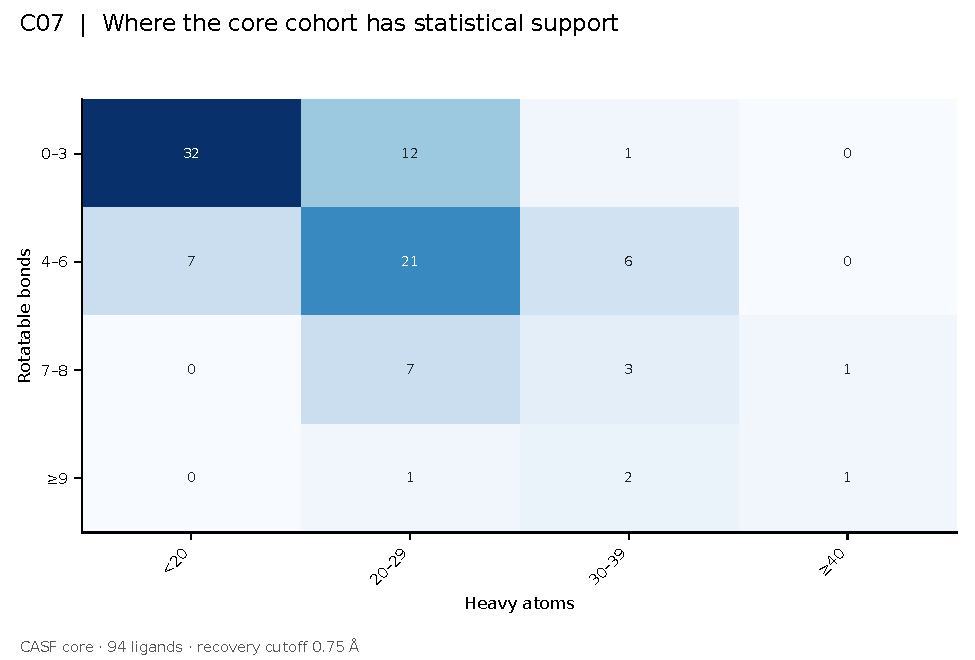
\includegraphics[width=\linewidth,height=0.72\textheight,keepaspectratio]{figures/candidates/c07-cohort-composition.pdf}
\caption{\textbf{Where the core cohort has statistical support.} Counts of the 94 core ligands cross-tabulated by heavy-atom and rotatable-bond groups using the same reference-derived descriptors for every method. Sparse large or flexible groups limit the stability of apparent method rankings. Size and flexibility are associated descriptors; this table does not isolate their independent effects.}
\label{fig:candidate-c07-cohort-composition}
\end{figure}
\clearpage
\begin{figure}[p]
\centering
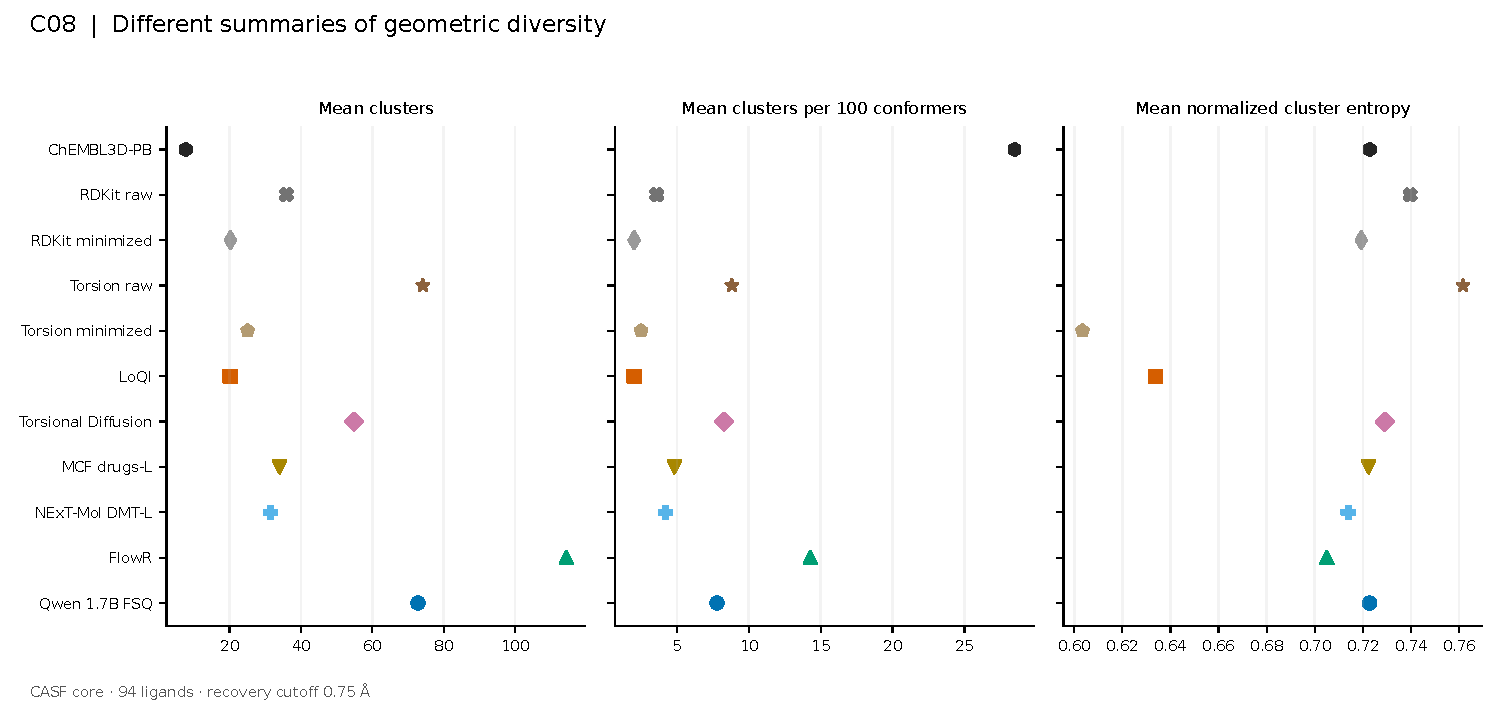
\includegraphics[width=\linewidth,height=0.72\textheight,keepaspectratio]{figures/candidates/c08-diversity-profiles.pdf}
\caption{\textbf{Different summaries of geometric diversity.} Per-ligand diversity summaries averaged over measurable core ensembles: cluster count, clusters per 100 conformers, and Shannon entropy divided by the logarithm of the number of occupied clusters (zero for a single cluster), at a 1.0~\AA{} clustering radius. This radius is distinct from the 0.75~\AA{} recovery cutoff. Generated pools use the 1,000-candidate target; ChEMBL3D-PB uses its finite pool. Normalizing cluster count does not fully remove sampling-size effects, and none of these metrics measures recovery by itself.}
\label{fig:candidate-c08-diversity-profiles}
\end{figure}
\clearpage
\begin{figure}[p]
\centering
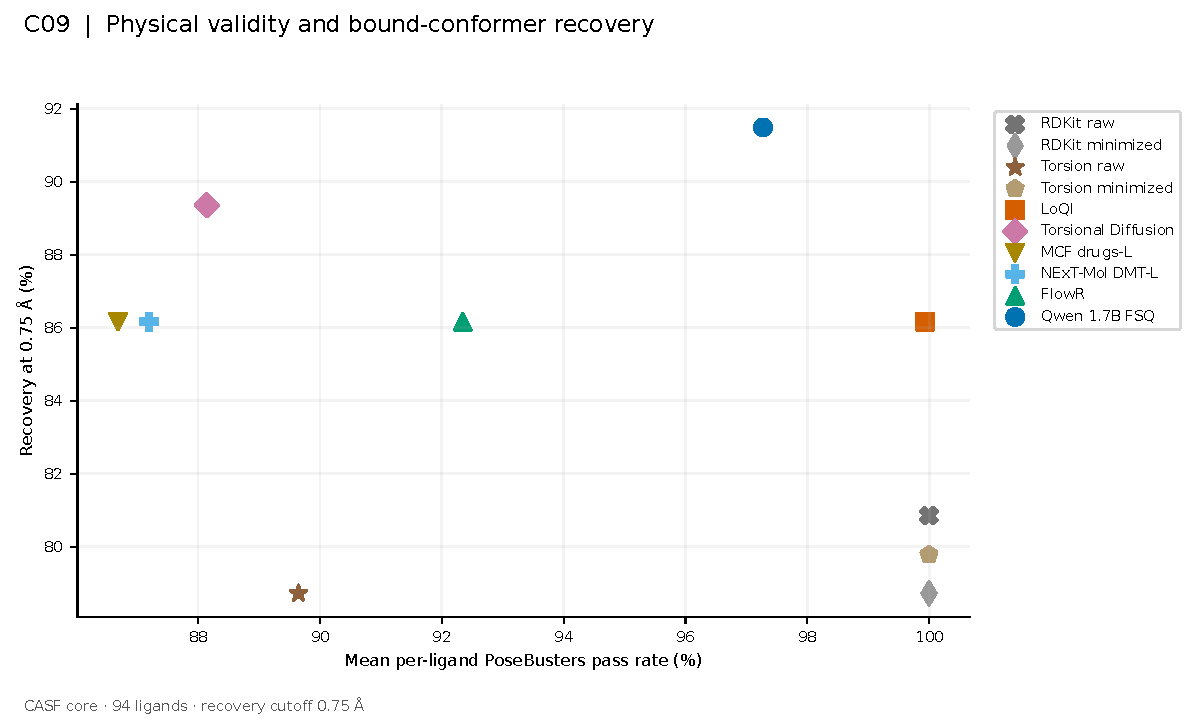
\includegraphics[width=\linewidth,height=0.72\textheight,keepaspectratio]{figures/candidates/c09-validity-recovery.pdf}
\caption{\textbf{Physical validity and bound-conformer recovery.} Mean per-ligand PoseBusters pass rate versus recovery for the ten generated core ensembles at the 1,000-candidate target. PoseBusters yield describes the analyzed input pools; it does not include every possible decoding or preprocessing rejection. Recovery requires a passing conformer and includes all 94 entries. High validity is a separate requirement from proximity to the observed bound conformation.}
\label{fig:candidate-c09-validity-recovery}
\end{figure}
\clearpage
\begin{figure}[p]
\centering
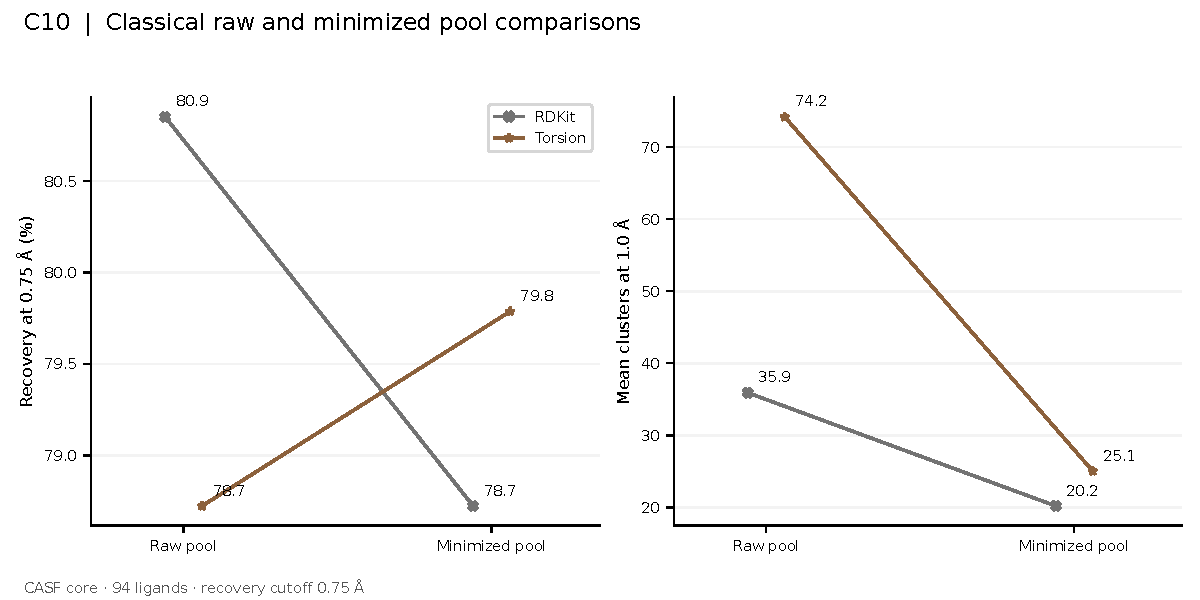
\includegraphics[width=\linewidth,height=0.72\textheight,keepaspectratio]{figures/candidates/c10-classical-pools.pdf}
\caption{\textbf{Classical raw and minimized pool comparisons.} Recovery and geometric diversity of RDKit and torsion-based raw and minimized core pools at the 1,000-candidate target. These are separately generated endpoint pools, not paired before-and-after measurements on identical conformers. Lines identify related pipelines and do not establish a causal effect of minimization. Diversity is averaged over measurable ensembles; recovery includes all core ligands.}
\label{fig:candidate-c10-classical-pools}
\end{figure}
\clearpage
\begin{figure}[p]
\centering
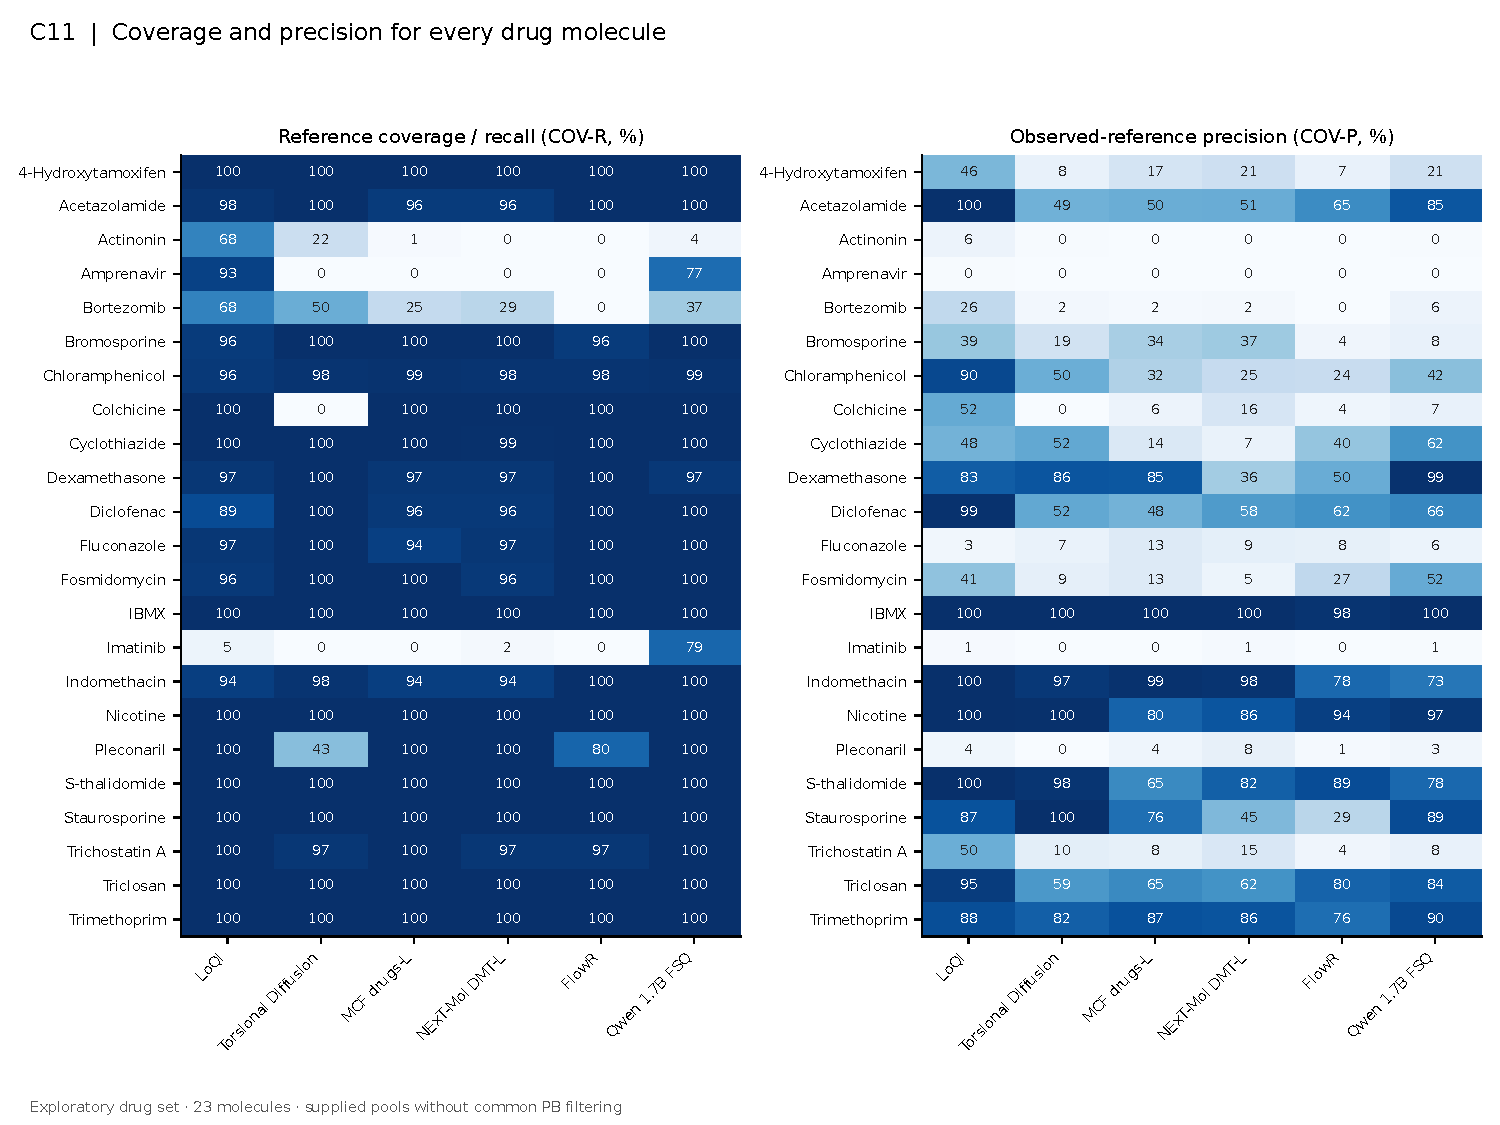
\includegraphics[width=\linewidth,height=0.72\textheight,keepaspectratio]{figures/candidates/c11-drug-coverage-matrix.pdf}
\caption{\textbf{Coverage and precision for every drug molecule.} Molecule-level COV-R and COV-P at the strict 0.75~\AA{} cutoff for all six selected generators. The two panels share a 0--100\% color scale. COV-R measures the fraction of observed references reached; COV-P measures the fraction of generated conformers near an observed reference. Unmatched conformers are not necessarily biologically impossible. All drug metrics describe supplied pools without a common PoseBusters mask; failed-RMSD handling also differs between imported evaluations. These are exploratory comparisons.}
\label{fig:candidate-c11-drug-coverage-matrix}
\end{figure}
\clearpage
\begin{figure}[p]
\centering
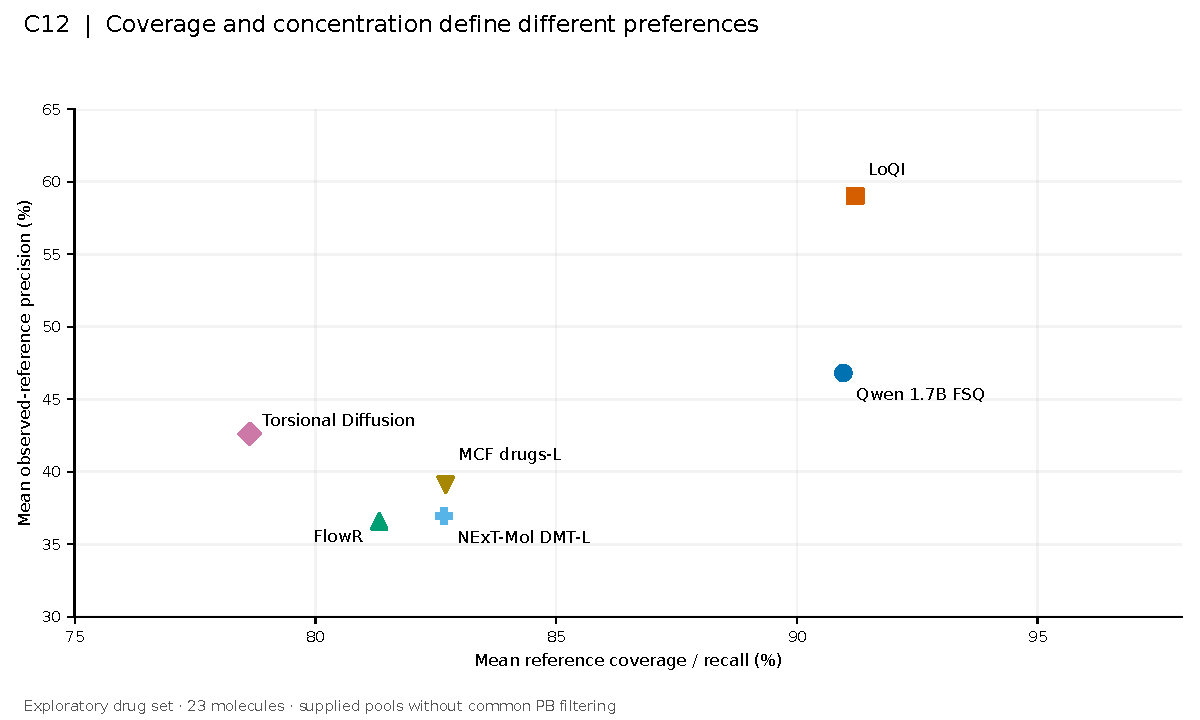
\includegraphics[width=\linewidth,height=0.72\textheight,keepaspectratio]{figures/candidates/c12-drug-tradeoff.pdf}
\caption{\textbf{Coverage and concentration define different preferences.} Molecule-mean recall and precision at 0.75~\AA{} for the six selected generators. Each of the 23 molecules receives equal weight regardless of its reference count. Higher values indicate broader observed-reference coverage or greater concentration near the available observations; they do not measure binding affinity or conformer populations. All drug metrics describe supplied pools without a common PoseBusters mask; failed-RMSD handling also differs between imported evaluations. These are exploratory comparisons.}
\label{fig:candidate-c12-drug-tradeoff}
\end{figure}
\clearpage
\begin{figure}[p]
\centering
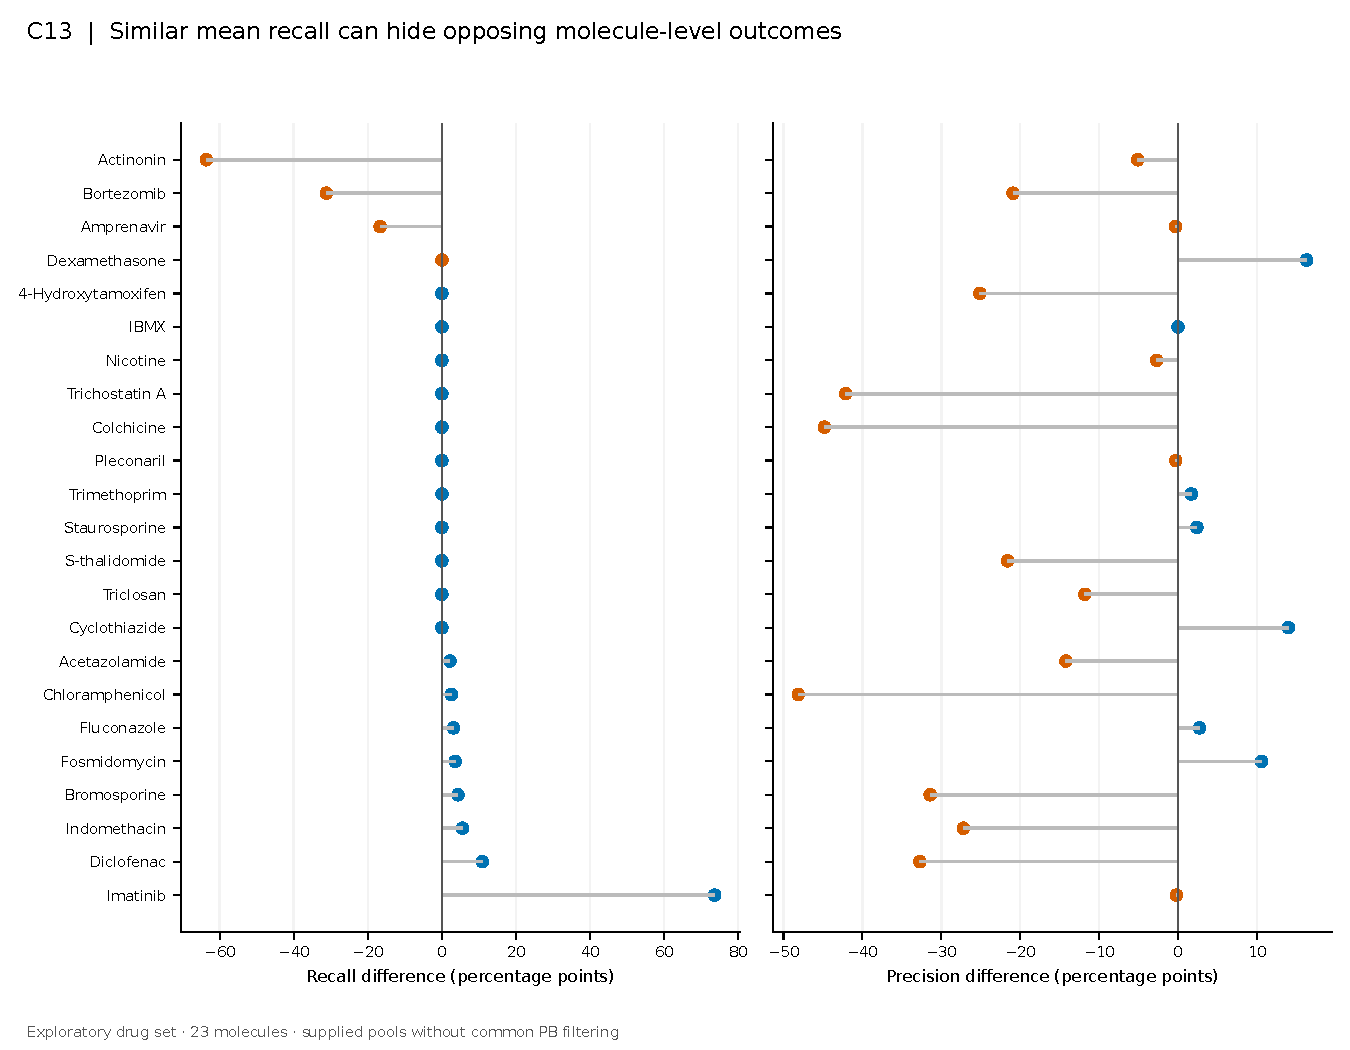
\includegraphics[width=\linewidth,height=0.72\textheight,keepaspectratio]{figures/candidates/c13-drug-paired-molecules.pdf}
\caption{\textbf{Similar mean recall can hide opposing molecule-level outcomes.} Paired molecule-level differences, Qwen 1.7B FSQ minus LoQI, in recall and precision at 0.75~\AA{}. Molecules are sorted by the recall difference and retain that ordering in both panels. Positive values favor Qwen, negative values favor LoQI. These descriptive differences are not per-molecule confidence intervals. All drug metrics describe supplied pools without a common PoseBusters mask; failed-RMSD handling also differs between imported evaluations. These are exploratory comparisons.}
\label{fig:candidate-c13-drug-paired-molecules}
\end{figure}
\clearpage
\begin{figure}[p]
\centering
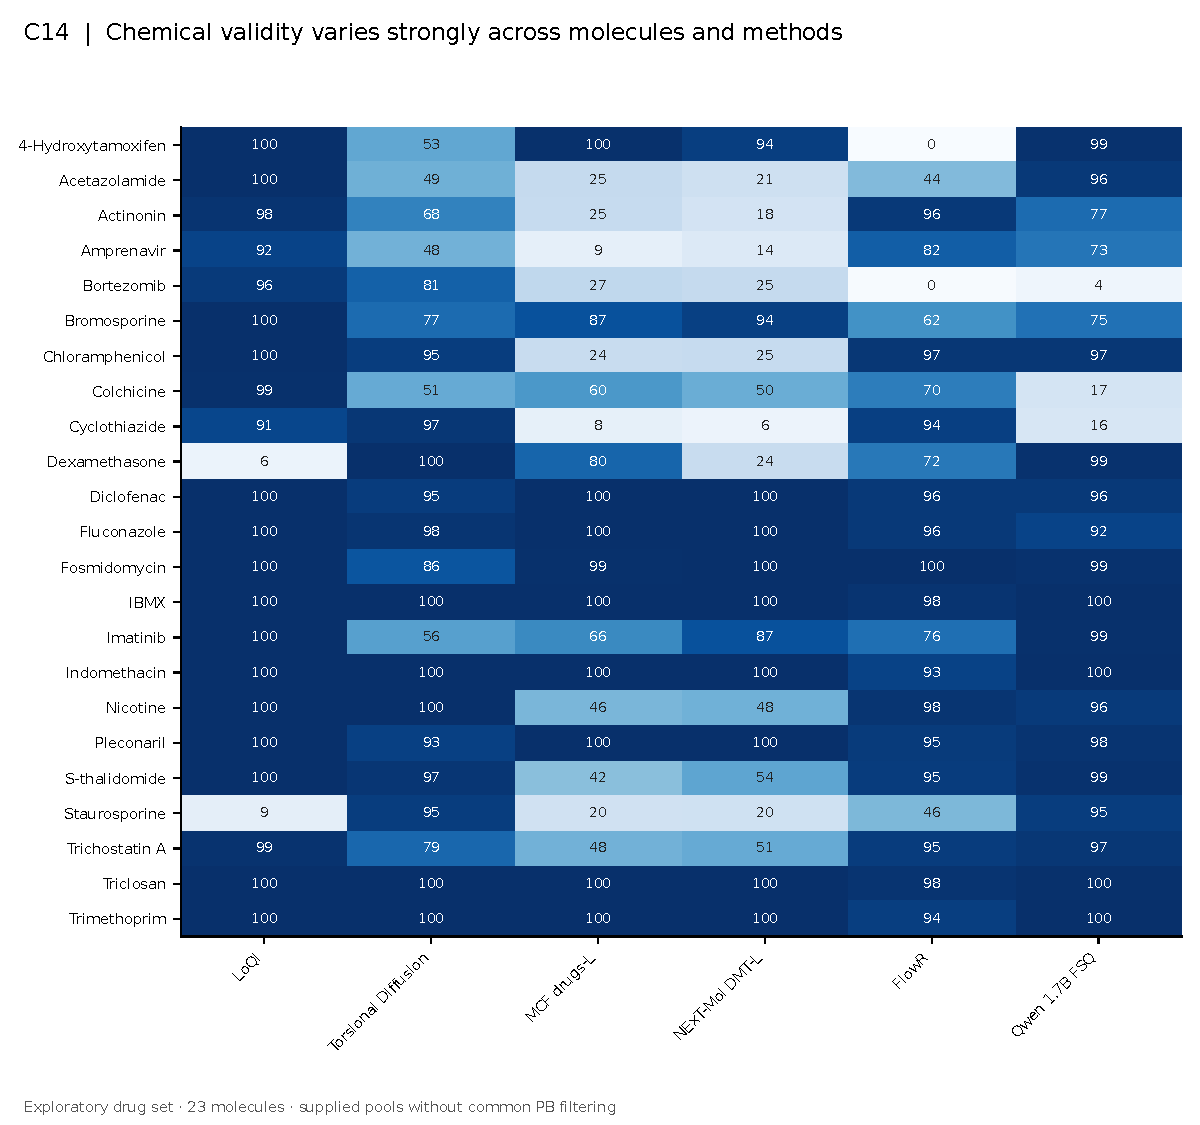
\includegraphics[width=\linewidth,height=0.72\textheight,keepaspectratio]{figures/candidates/c14-drug-validity.pdf}
\caption{\textbf{Chemical validity varies strongly across molecules and methods.} PoseBusters pass percentages for each supplied drug molecule--method pool. The common color scale spans 0--100\%. Validity is reported separately from coverage and precision: coverage cannot be adjusted by multiplying it by these percentages because the passing conformers and recovered references need not coincide. All drug metrics describe supplied pools without a common PoseBusters mask; failed-RMSD handling also differs between imported evaluations. These are exploratory comparisons.}
\label{fig:candidate-c14-drug-validity}
\end{figure}
\clearpage
\begin{figure}[p]
\centering
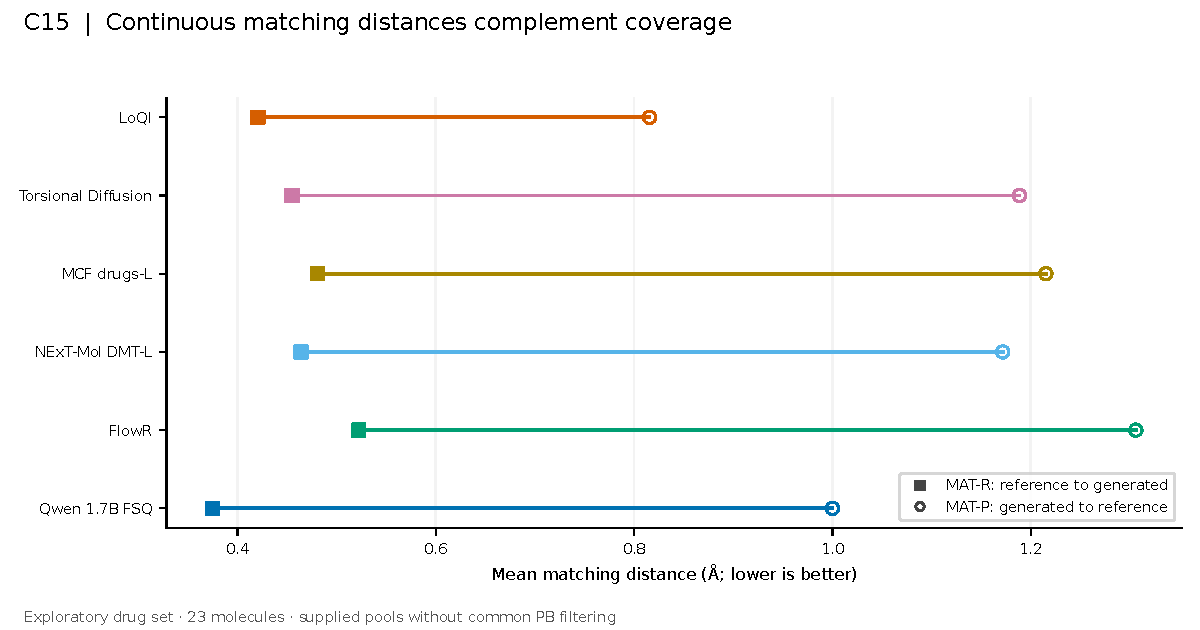
\includegraphics[width=\linewidth,height=0.72\textheight,keepaspectratio]{figures/candidates/c15-drug-matching-distance.pdf}
\caption{\textbf{Continuous matching distances complement coverage.} Molecule-mean MAT-R and MAT-P for the six selected generators. MAT-R averages nearest generated-conformer distances from observed references; MAT-P averages nearest observed-reference distances from generated conformers. Lower is better. Segments connect distinct summaries rather than uncertainty bounds. All drug metrics describe supplied pools without a common PoseBusters mask; failed-RMSD handling also differs between imported evaluations. These are exploratory comparisons.}
\label{fig:candidate-c15-drug-matching-distance}
\end{figure}
\clearpage
\begin{figure}[p]
\centering
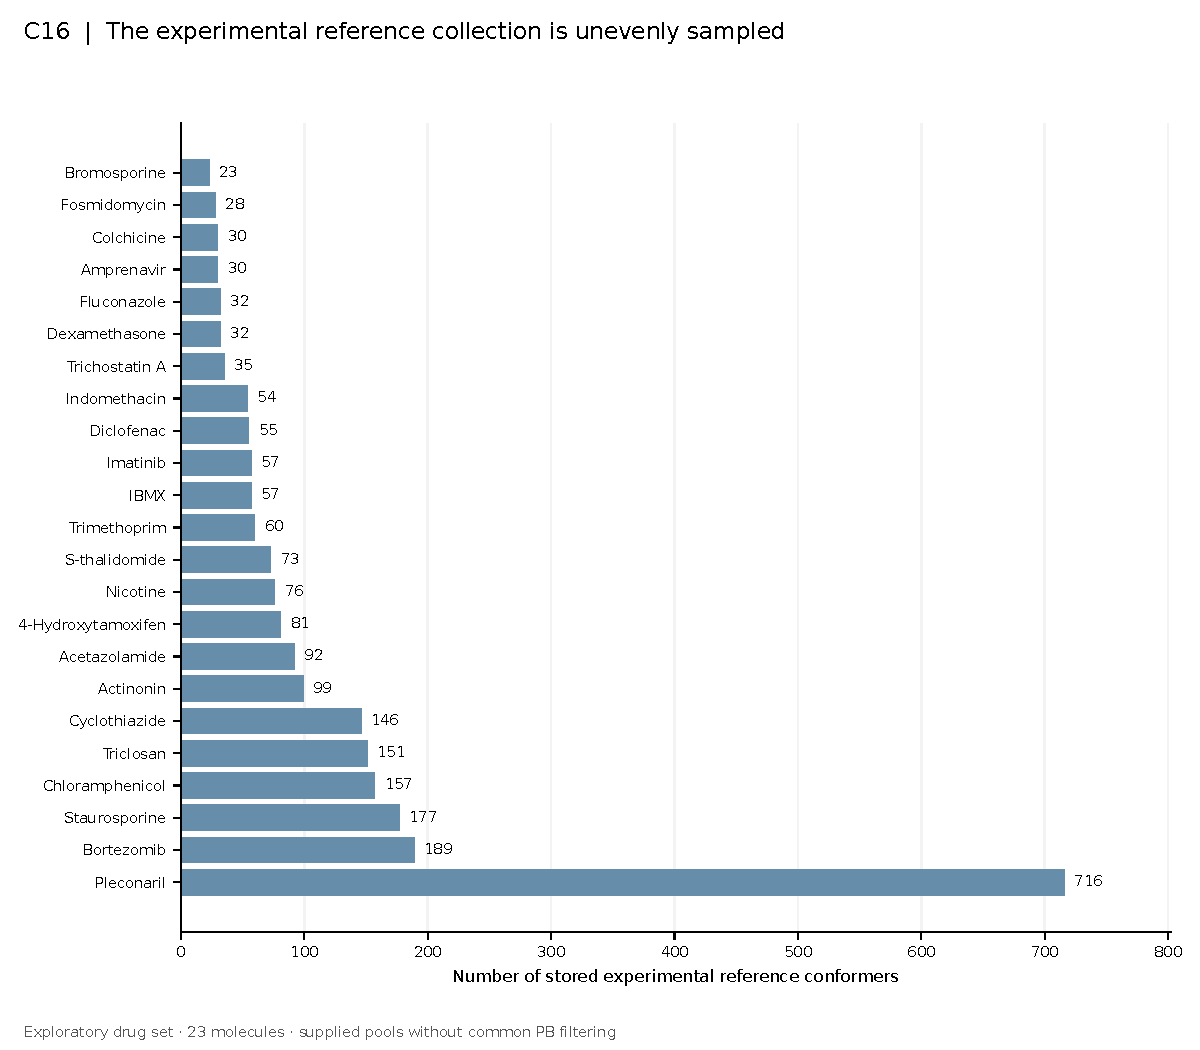
\includegraphics[width=\linewidth,height=0.72\textheight,keepaspectratio]{figures/candidates/c16-drug-reference-counts.pdf}
\caption{\textbf{The experimental reference collection is unevenly sampled.} Numbers of stored experimental reference conformers for the 23 drug molecules (2,450 in total). Reference counts are not counts of unique conformational states: redundant or very similar geometries may recur. Reported coverage and precision aggregates average molecules equally, so reference-rich molecules do not receive extra aggregate weight.}
\label{fig:candidate-c16-drug-reference-counts}
\end{figure}
\clearpage
\begin{figure}[p]
\centering
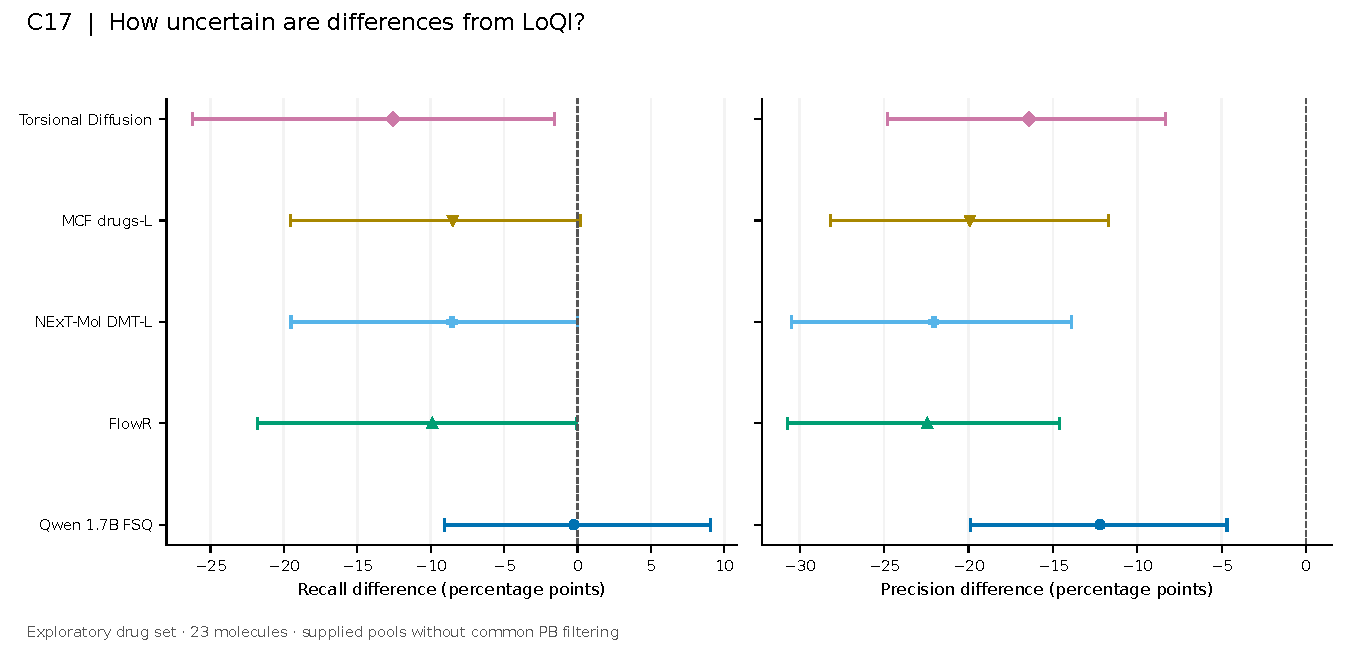
\includegraphics[width=\linewidth,height=0.72\textheight,keepaspectratio]{figures/candidates/c17-drug-paired-uncertainty.pdf}
\caption{\textbf{How uncertain are differences from LoQI?.} Paired differences from LoQI in molecule-mean COV-R and COV-P at 0.75~\AA{}. Error bars are exploratory 95\% percentile intervals from 10,000 paired molecule bootstrap samples (23 molecules; seed 20260928). These newly rendered intervals can differ slightly from earlier exports because the resampling seed differs. Intervals are not adjusted for multiple comparisons; an interval crossing zero does not establish equivalence. All drug metrics describe supplied pools without a common PoseBusters mask; failed-RMSD handling also differs between imported evaluations. These are exploratory comparisons.}
\label{fig:candidate-c17-drug-paired-uncertainty}
\end{figure}
\clearpage
\begin{figure}[p]
\centering
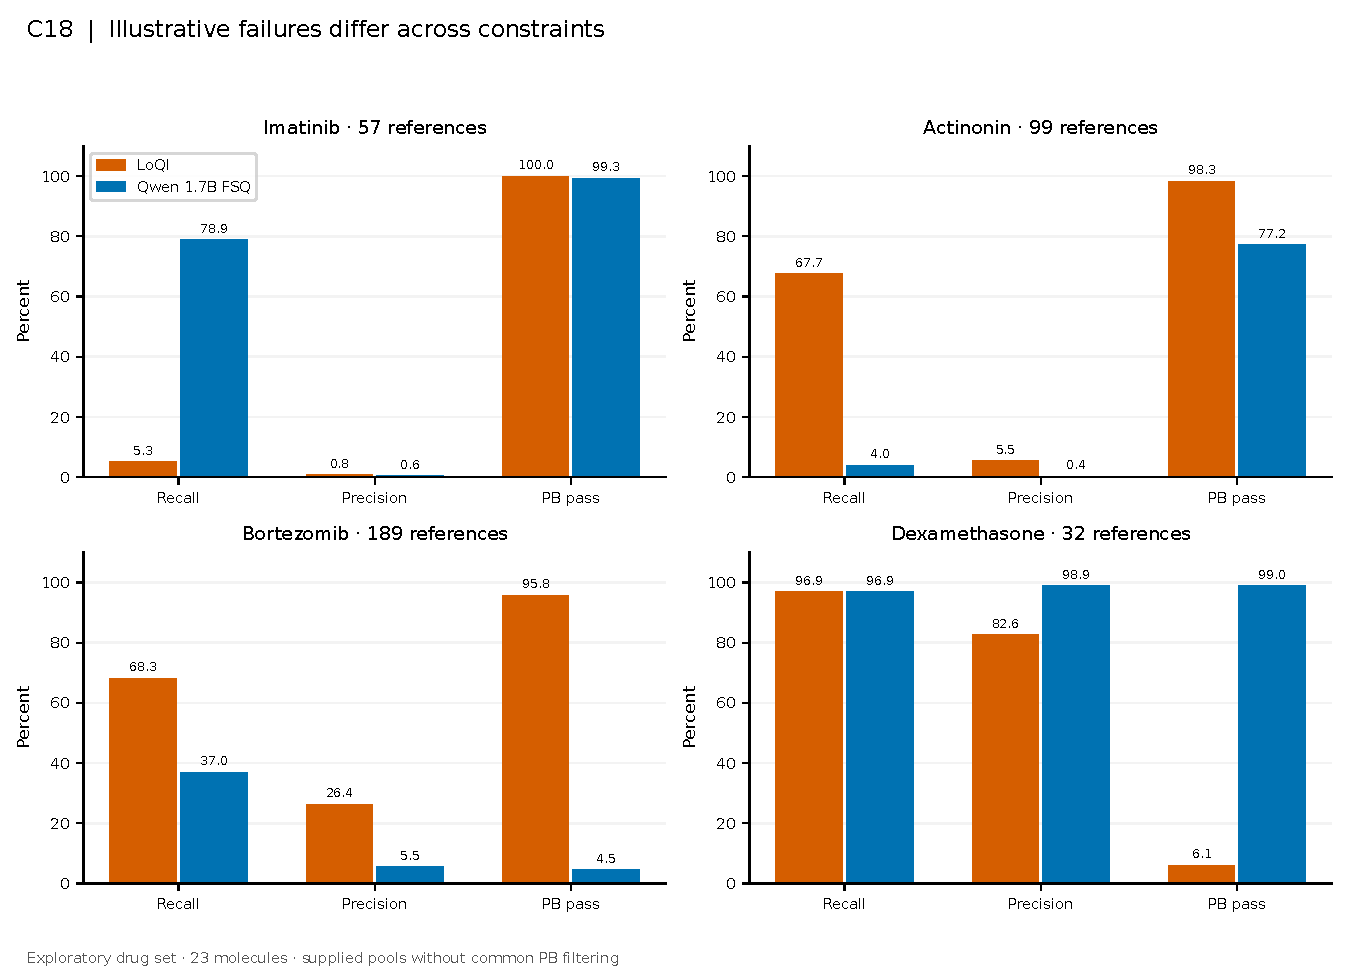
\includegraphics[width=\linewidth,height=0.72\textheight,keepaspectratio]{figures/candidates/c18-drug-case-profiles.pdf}
\caption{\textbf{Illustrative failures differ across constraints.} Four post hoc illustrative molecules comparing LoQI and Qwen 1.7B FSQ: recall, precision, and PoseBusters pass rate. Coverage uses the strict 0.75~\AA{} cutoff. The cases illustrate opposing recall preferences and disagreements between geometric coverage and chemical validity; they are not a representative sample or a structural explanation. All drug metrics describe supplied pools without a common PoseBusters mask; failed-RMSD handling also differs between imported evaluations. These are exploratory comparisons.}
\label{fig:candidate-c18-drug-case-profiles}
\end{figure}
\clearpage
\endgroup
